\subsection{The Multivariate Oxide Composition Model}\label{sec:moc}
\begin{figure}[H]
    \centering
    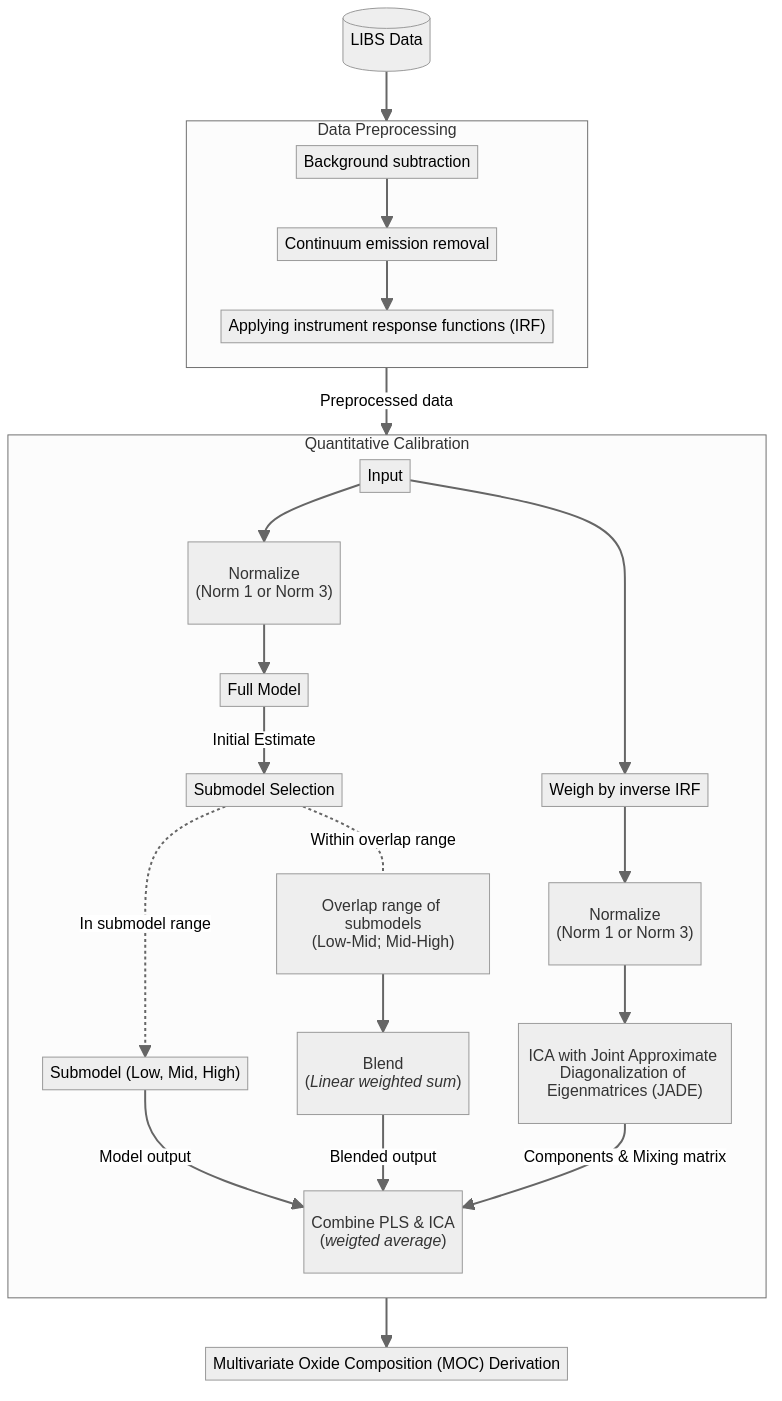
\includegraphics[width=0.45\textwidth]{images/pipeline.png}
    \caption{Flowchart illustrating the data processing and calibration steps for Laser-Induced Breakdown Spectroscopy (LIBS) data leading to the derivation of Multivariate Oxide Composition (MOC).}
    \label{fig:libs_data_processing}
\end{figure}

We illustrate the data processing and calibration steps for LIBS data leading to the derivation of Multivariate Oxide Composition (MOC) in Figure \ref{fig:libs_data_processing}. The MOC model is described in details by \citet{cleggRecalibrationMarsScience2017} and \citet{andersonImprovedAccuracyQuantitative2017}, but we provide a brief overview here, which will serve as a foundation for the subsequent discussion of our work.

\subsection{Data Preprocessing}\label{sec:data_preprocessing}

The initial phase of processing the raw emission data records (EDR) involves a series of steps to clean up the spectra for subsequent analysis.
The pipeline, as illustrated in Figure \ref{fig:libs_data_processing}, commences with the subtraction of the dark spectrum.
This step is crucial to isolate the signal emanating solely from the plasma, thereby removing the effects of ambient light and reflected sunlight that are present when the laser is not employed.

To further refine the spectra, an undecimated wavelet transform is applied.
This advanced signal processing technique effectively reduces noise while preserving the essential features of the spectrum.
The subsequent wavelength calibration ensures the precise alignment of spectra by compensating for wavelength shifts as a function of temperature across every pixel.

A critical step in preprocessing is the removal of the continuum, which predominantly arises from Bremsstrahlung emission and ion recombination.
The continuum is subtracted because it carries minimal information pertinent to the target material's composition.
The processed data, at this stage, is referred to as the reduced data record (RDR).

The final step in data preparation involves the conversion of the spectral data from counts to photons by applying an instrument response function (IRF) correction.
This yields a set of cleaned and calibrated spectra (CCS), primed for the subsequent compositional analysis.

\subsection{Multivariate Oxide Composition Derivation}\label{sec:moc_derivation}

The multivariate analysis employs a composite approach integrating partial least squares regression with submodels (PLS-SM) and independent component analysis (ICA) to derive the Multivariate Oxide Composition (MOC).
The PLS-SM approach utilizes tailored sub-models for distinct composition ranges, enhancing accuracy at the boundaries of these ranges.
Independent Component Analysis assists in distinguishing elemental emission lines, contributing to a refined multivariate model.

Two normalization methods are employed in the analysis: Norm 1 and Norm 3.
Norm 1 standardizes the full spectrum across all three spectrometers such that the sum total is unity.
In contrast, Norm 3 conducts normalization on a per-spectrometer basis, culminating in a full normalized spectrum summing to three.
The optimal normalization technique is selected based on its efficacy in model performance for the specific analysis task at hand.

\subsubsection{Outlier Removal}\label{sec:outlier_removal}

In the critical phase of outlier removal, our approach is grounded in the iterative refinement of the PLS model, informed by influence plots.
These plots offer a visual domain to distinguish outliers based on spectral residuals and leverage, a methodical way to weed out spectral anomalies.
This iterative process is essential for the model's integrity, ensuring that each spectrum contributes constructively to the analytical framework.
Outliers, discerned through their disproportionate influence or aberrant residuals, are prudently removed, thereby preserving the model's fidelity to the majority of the data that adhere to expected statistical patterns.


\subsubsection{Partial Least Squares Sub-Models}\label{sec:pls_submodels}

The implementation of sub-models in PLS regression, as described by \citet{andersonImprovedAccuracyQuantitative2017}, serves to fine-tune the model's performance across varying levels of elemental composition in geological samples. This is done by training distinct models on sub-sets of data that represent low, medium, and high concentration ranges. The sub-models' concentration ranges overlap to ensure a smooth transition between predictions, thus avoiding abrupt shifts in accuracy that can occur when switching from one model's range to another.

The integration of these sub-models is achieved through a process called blending, where the initial estimate of composition made by a full-range model determines which sub-models are applied for the final prediction. If the estimate falls within the extreme ranges (low or high), the respective sub-model is used exclusively. However, if it lies within the overlapping ranges (low-mid or mid-high), the final prediction is a weighted blend of the two relevant sub-model predictions.

The weights for blending are calculated such that the closer the initial full-range estimate is to a sub-model's specific range, the more influence that sub-model has on the final prediction. This weighting ensures that the transition across the composition spectrum is gradual and cohesive.

\citet{andersonImprovedAccuracyQuantitative2017} used the Broyden-Fletcher-Goldfarb-Shanno (BFGS) optimization algorithm to ascertain the most effective blending ranges. This method iteratively adjusts the blending boundaries to minimize the root mean square error (RMSE) on the training set, leading to the refined performance of the overall model.

In practical terms, these sub-models, when correctly optimized and blended, allow for precise predictions over a broad range of elemental compositions, providing robust and accurate analytical capabilities for the evaluation of geological samples through chemometric methods.

\subsubsection{Independent Component Analysis}\label{sec:ica}

The ICA implementation via the Joint Approximate Diagonalization of Eigenmatrices (JADE) algorithm provides a robust mechanism for separating mixed signals into their independent components.
By focusing on higher-order statistical independence rather than merely uncorrelatedness, the JADE algorithm offers a powerful tool for uncovering the fundamental emission lines within the spectral data, which are essential for accurate composition analysis.

In summary, the detailed pipeline for LIBS data processing and analysis integrates a comprehensive suite of preprocessing, multivariate analysis, and optimization techniques, as delineated in the process flow of Figure \ref{fig:libs_data_processing}.
The harmonized use of PLS-SM, ICA, and meticulous outlier management culminates in a robust method for quantifying the oxide composition of the studied materials.